\title{8-bit comparator design}
\author{
        Maxim Blumental \\
                VLSI project\\
        \\
}
\date{\today}

\documentclass[12pt]{article}
\usepackage{circuitikz}
\usepackage{tikz}
\usetikzlibrary{circuits.logic.US,calc}
\begin{document}
\maketitle

\begin{abstract}
My colleges (Alexander Kravtsov and Marina Shimchenko) and me made some estimations based on which we came up with a design of 8-bit comparator. The paper contains a brief report about the results.
\end{abstract}

\section{Underlying boolean function}

As we know, XOR operation returns 'true' when its input bits are different. So, conjunction of negated XOR's for every bit pair would serve nicely as the required function:

$$\lnot (A_0 \oplus B_0) \land  \lnot (A_1 \oplus B_1) ... \land  \lnot (A_7 \oplus B_7)$$

\section{Truth table}

Let's illustrate that by 1-bit case:

\
\begin{tabular}{|r|l|c|}
  \hline
  $A_0$ & $B_0$ & $\lnot (A_0 \oplus B_0)$ \\
  \hline
  0 & 0 & 1 \\
  0 & 1 & 0 \\
  1 & 0 & 0 \\
  1 & 1 & 1 \\
  \hline
\end{tabular}

\

As you can see, 'truth' when bits are equal. The results for each bit are AND'ed then.
\section{Logical scheme}
Let's illustrate the idea with 2-bit comparator scheme:

\begin{circuitikz} \draw
(0,2) node[xnor port] (myxnor1) {}
(0,0) node[xnor port] (myxnor2) {}
(2,1) node[and port] (myand) {}
(myxnor1.out) -| (myand.in 1)
(myxnor2.out) -| (myand.in 2)
;\end{circuitikz}

However, in our case we need AND gate with 8 inputs. We've decided to implement AND8 as a combination of simpler gates - two NAND4 and one NOR2:

\

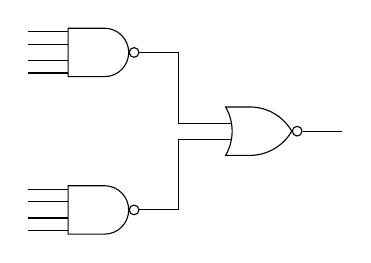
\begin{tikzpicture}[circuit logic US]
\draw (0,0) node[nand gate](NAND1){}
  ($(NAND1.north west)!.25!(NAND1.input 1)$) -- +(-.5,0)
  (NAND1.input 1) -- +(-.5,0)
  (NAND1.input 2) -- +(-.5,0)
  ($(NAND1.south west)!.25!(NAND1.input 2)$) -- +(-.5,0);
\draw  (0,2) node[nand gate](NAND2){}
  ($(NAND2.north west)!.25!(NAND2.input 1)$) -- +(-.5,0)
  (NAND2.input 1) -- +(-.5,0)
  (NAND2.input 2) -- +(-.5,0)
  ($(NAND2.south west)!.25!(NAND2.input 2)$) -- +(-.5,0);
\draw  (2,1) node[nor gate](XNOR2){}
  (NAND1.output) -- +(.5,0) |- (XNOR2.input 2)
  (NAND2.output) -- +(.5,0) |- (XNOR2.input 1)
  (XNOR2.output) -- +(.5,0);
\end{tikzpicture}

\section{Delay estimation with practical method}
According to the Gold table:

$$t_{NGD} = t_{XNOR} + t_{NAND4} + t_{NOR2} = 1.3 + 1.1 + 1.4 = 3.8 $$


\section{Optimal delay estimation with LE method}

Logical effort: $G = g_{XNOR} * g_{NAND4} * g_{NOR2} = 4 * \frac{6}{3} * \frac{5}{3} = \frac{40}{3}$

\paragraph{a: H=50}

\

Path effort: $F_a = GH = \frac{40}{3} * 50 = 666 \frac{2}{3}$.

Best number of stages: $N_a = log_{4}F_a \approx 4.69$

\paragraph{b: H=1000}

\


Path effort: $F_b = GH = \frac{40}{3} * 1000 = 13333 \frac{1}{3}$.

Best number of stages: $N_b = log_{4}F_b \approx 6.85$

\paragraph{So what?}

\

Now we have to analyze four situations, two for each value of H: $N=4$ and $N=5$ for $H=50$; $N=6$ and $N=7$ for $H=1000$. Each situation requires the initial logic scheme (see paragraph \textbf{Logical scheme}) to be adjusted so that the amount of stages was correspondent.

\paragraph{Case 1: H=50, N=4}
\

The critical path:

\begin{circuitikz} \draw
(0,2) node[xor port] (myxor) {}
(1,1.28) node[not port] (mynot) {}
(3,1) node[nand port] (mynand) {}
(5,0) node[nor port] (mynor) {}
(myxor.out) -| (mynot.in)
(mynot.out) -| (mynand.in 1)
(mynand.out) -| (mynor.in 1)
;\end{circuitikz}

(imagine that NAND has four inputs on the figure)

\

Logical effort $G$: doesn't change ($g_{inv}=1$).

The least delay: $\hat{f} = F^{\frac{1}{N}} = (666 \frac{2}{3})^{\frac{1}{4}} \approx 5.08\tau $

Parasitic delay: $P = p_{XOR} + p_{NOT} + p_{NAND4} + p_{NOR2} = 4 + 1 + 4 + 2 = 11\tau$

Path delay: $D = N\hat{f}+P = 4*5.08+11 = 31.32\tau = 5.22 NGD$

\paragraph{Case 2: H=50, N=5}
\

The critical path:

\begin{circuitikz} \draw
(0,2) node[xnor port] (myxnor) {}
(1,1.275) node[not port] (mynot1) {}
(3,1) node[nand port] (mynand) {}
(4,1) node[not port] (mynot2) {}
(7,0) node[nor port] (mynor) {}
(myxnor.out) -| (mynot1.in)
(mynot.out) -| (mynand.in 1)
(mynand.out) -| (mynot2.in)
(mynot2.out) -| (mynor.in 1)
;\end{circuitikz}

(again: the NAND is NAND4)

\

Logical effort $G$: doesn't change ($g_{inv}=1$).

The least delay: $\hat{f} = F^{\frac{1}{N}} = (666 \frac{2}{3})^{\frac{1}{5}} \approx 3.67\tau $

Parasitic delay: $P = p_{XNOR} + 2*p_{NOT} + p_{NAND4} + p_{NOR2} = 4 + 2 + 4 + 2 = \ = 12\tau$

Path delay: $D = N\hat{f}+P = 5*3.67+12 = 30.35\tau = 5.06 NGD$

\paragraph{Case 3: H=1000, N=6}
\

The critical path:

\begin{circuitikz} \draw
(0,2) node[xor port] (myxor) {}
(1,1.275) node[not port] (mynot1) {}
(2.5,1.275) node[not port] (mynot2) {}
(5,1) node[nand port] (mynand) {}
(6,1) node[not port] (mynot3) {}
(8.5,0) node[nor port] (mynor) {}
(myxor.out) -| (mynot1.in)
(mynot1.out) -| (mynot2.in)
(mynot2.out) -| (mynand.in 1)
(mynand.out) -| (mynot3.in)
(mynot3.out) -| (mynor.in 1)
;\end{circuitikz}

(still NAND4...)

\

Logical effort $G$: doesn't change ($g_{inv}=1$).

The least delay: $\hat{f} = F^{\frac{1}{N}} = (13333 \frac{1}{3})^{\frac{1}{6}} \approx 4.87\tau $

Parasitic delay: $P = p_{XOR} + 3*p_{NOT} + p_{NAND4} + p_{NOR2} = 4 + 3 + 4 + 2 = \ = 13\tau$

Path delay: $D = N\hat{f}+P = 6*4.87+13 = 42.22\tau = 7.04 NGD$

\paragraph{Case 4: H=1000, N=7}
\

The critical path:

\begin{circuitikz} \draw
(0,2) node[xnor port] (myxnor) {}
(1,1.275) node[not port] (mynot1) {}
(2.5,1.275) node[not port] (mynot2) {}
(5,1) node[nand port] (mynand) {}
(6,1) node[not port] (mynot3) {}
(7.5,1) node[not port] (mynot4) {}
(10,0) node[nor port] (mynor) {}
(myxnor.out) -| (mynot1.in)
(mynot1.out) -| (mynot2.in)
(mynot2.out) -| (mynand.in 1)
(mynand.out) -| (mynot3.in)
(mynot3.out) -| (mynot4.in)
(mynot4.out) -| (mynor.in 1)
;\end{circuitikz}

(NAND4 - das Auto)

\

Logical effort $G$: doesn't change ($g_{inv}=1$).

The least delay: $\hat{f} = F^{\frac{1}{N}} = (13333 \frac{1}{3})^{\frac{1}{7}} \approx 3.88\tau $

Parasitic delay: $P = p_{XNOR} + 4*p_{NOT} + p_{NAND4} + p_{NOR2} = 4 + 4 + 4 + 2 = \ = 14\tau$

Path delay: $D = N\hat{f}+P = 7*3.88+14 = 41.16\tau = 6.86 NGD$

\paragraph{Conclusion:}
\

Optimal stage numbers are: 1) $N=5$;  2) $N=7$.

\end{document}